\subsection{Plots of observed and fitted frequencies}
Plots of the observed and fitted frequencies can help to show
both the shape of the theoretical distribution we have fitted and the
pattern of any deviations between our data and theory.

\figref{fig:madfit1} shows the fit of the Poisson distribution to the Federalist papers data, using one common form of plot that is sometimes
used for this purpose.
In this plot, observed frequencies are shown by bars and fitted
frequencies are shown by points, connected by a smooth (spline)
curve.%
%\footnote{Using a curve has the unfortunate }

Such a plot, however, is dominated by the largest frequencies,
making it hard to assess the deviations among the smaller frequencies.
To make the smaller frequencies more visible, \citet{Tukey:77}
suggest plotting the frequencies  on a square-root scale,
which he calls a \emph{rootogram} (see \figref{fig:madfit2}).
An additional improvement is to move the rootogram bars so their tops
are at the expected frequencies (giving a \emph{hanging rootogram}, \figref{fig:madfit3}).
This has the advantage that we can more easily judge the pattern
of departures against the horizontal reference line at 0, than
against the curve.
A final variation is to emphasize the differences between the
observed and fitted frequencies by drawing the bars to show the
gaps between the 0 line and the (observed-expected) difference
(\figref{fig:madfit4}).

These plots are produced by the \macro{ROOTGRAM} using the (default)
\texttt{OUT=FIT}
\Dset\ from the \macro{GOODFIT}:
%% input: /users/faculty/friendly/sasuser/catdata/madfit.sas
%% last modified: 08-Apr-99  8:31
\begin{listing}
title "Instances of 'may' in Federalist papers" ;
%include catdata(madison);
%goodfit(data=madison, var=count, freq=blocks, dist=poisson, out=fit);

title;
%rootgram(data=fit, var=count, obs=blocks, btype=0, func=none);  /* a */
%rootgram(data=fit, var=count, obs=blocks, btype=0);             /* b */
%rootgram(data=fit, var=count, obs=blocks);                      /* c */
%rootgram(data=fit, var=count, obs=blocks, btype=dev);           /* d */
\end{listing}


% subfigmatrix 2 x 2
\begin{figure}[htb]
 \begin{subfigmatrix}{2}
 \subfigure[Histogram]{\label{fig:madfit1}%
  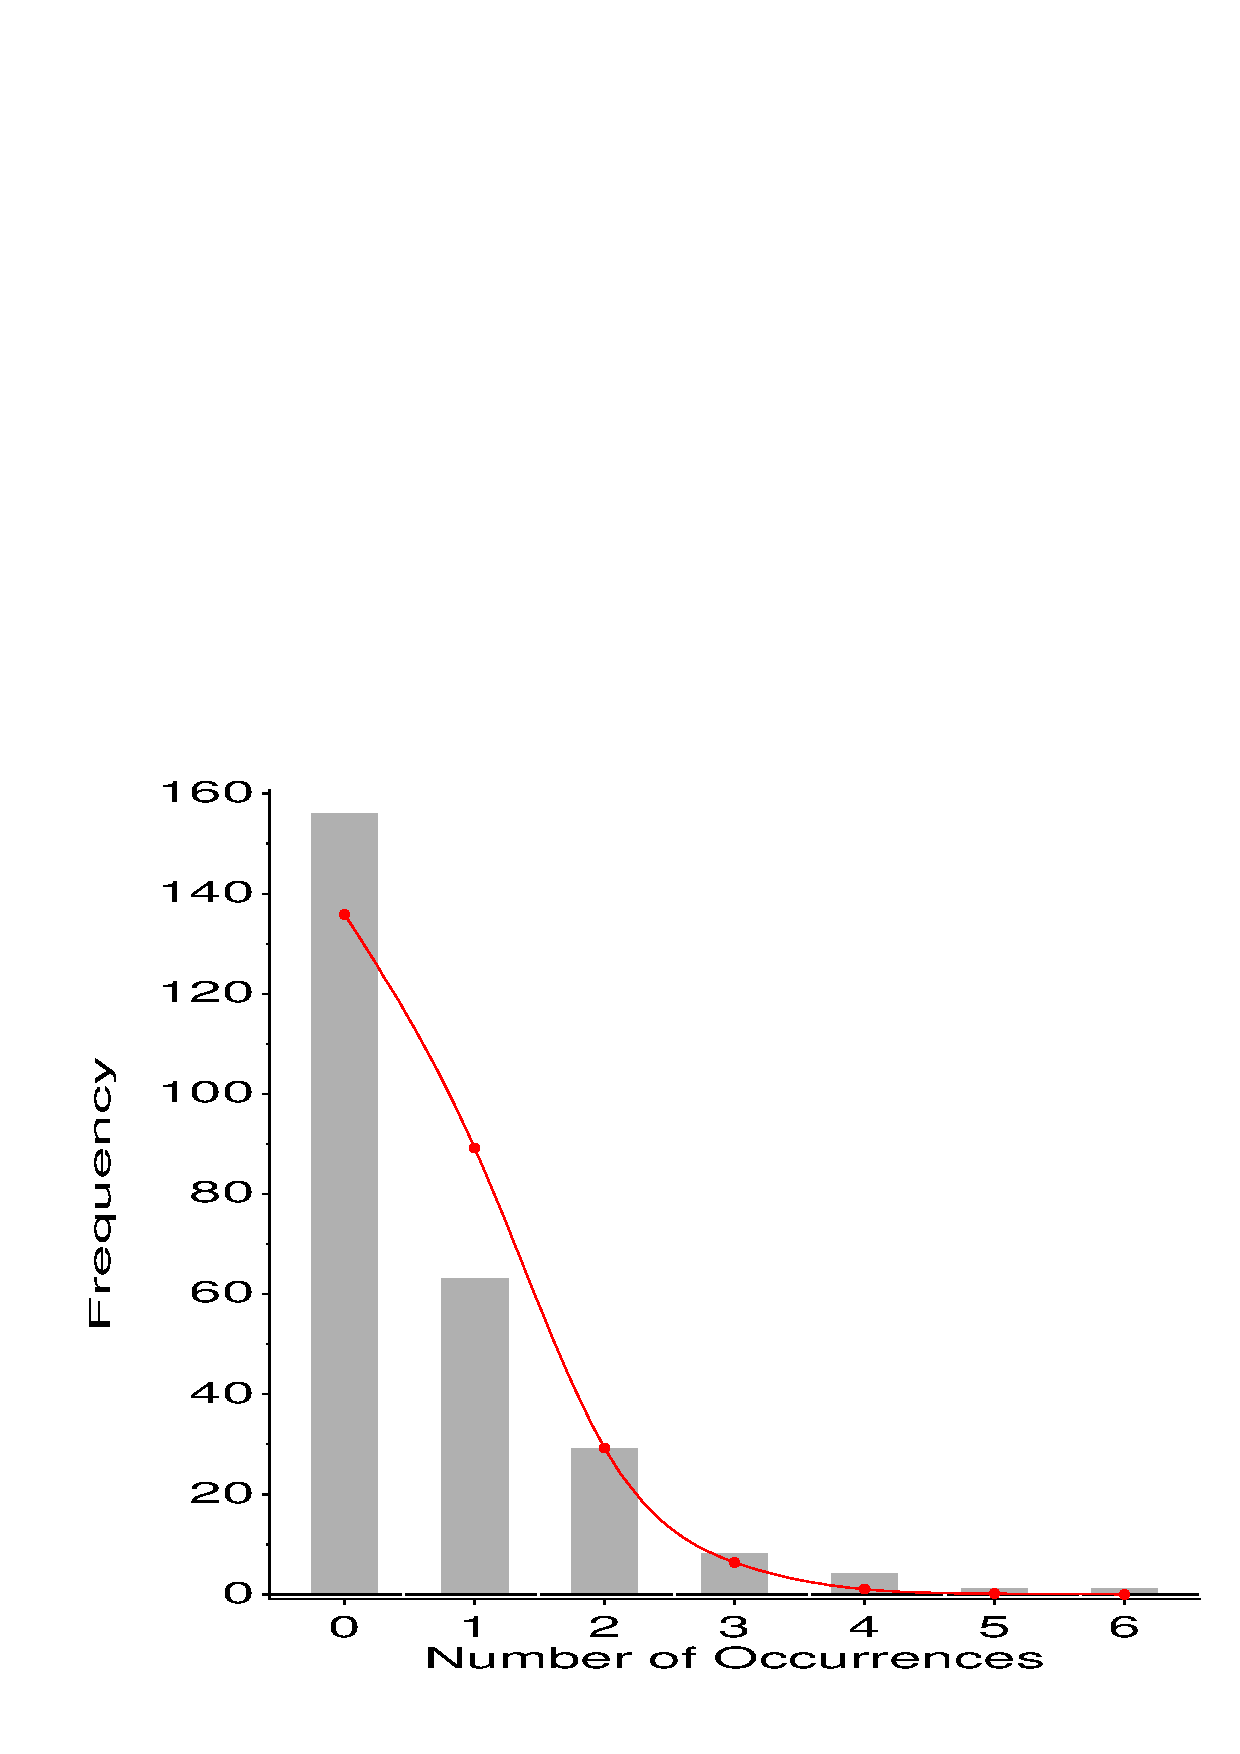
\includegraphics{madfit1}\graphicsfile{ch2/fig/madfit1.eps}{}
 }
 \subfigure[Rootogram]{\label{fig:madfit2}%
  \includegraphics{madfit2}\graphicsfile{ch2/fig/madfit2.eps}{}
 }
 \subfigure[Hanging rootogram]{\label{fig:madfit3}%
  \includegraphics{madfit3}\graphicsfile{ch2/fig/madfit3.eps}{}
 }
 \subfigure[Deviation rootogram]{\label{fig:madfit4}%
  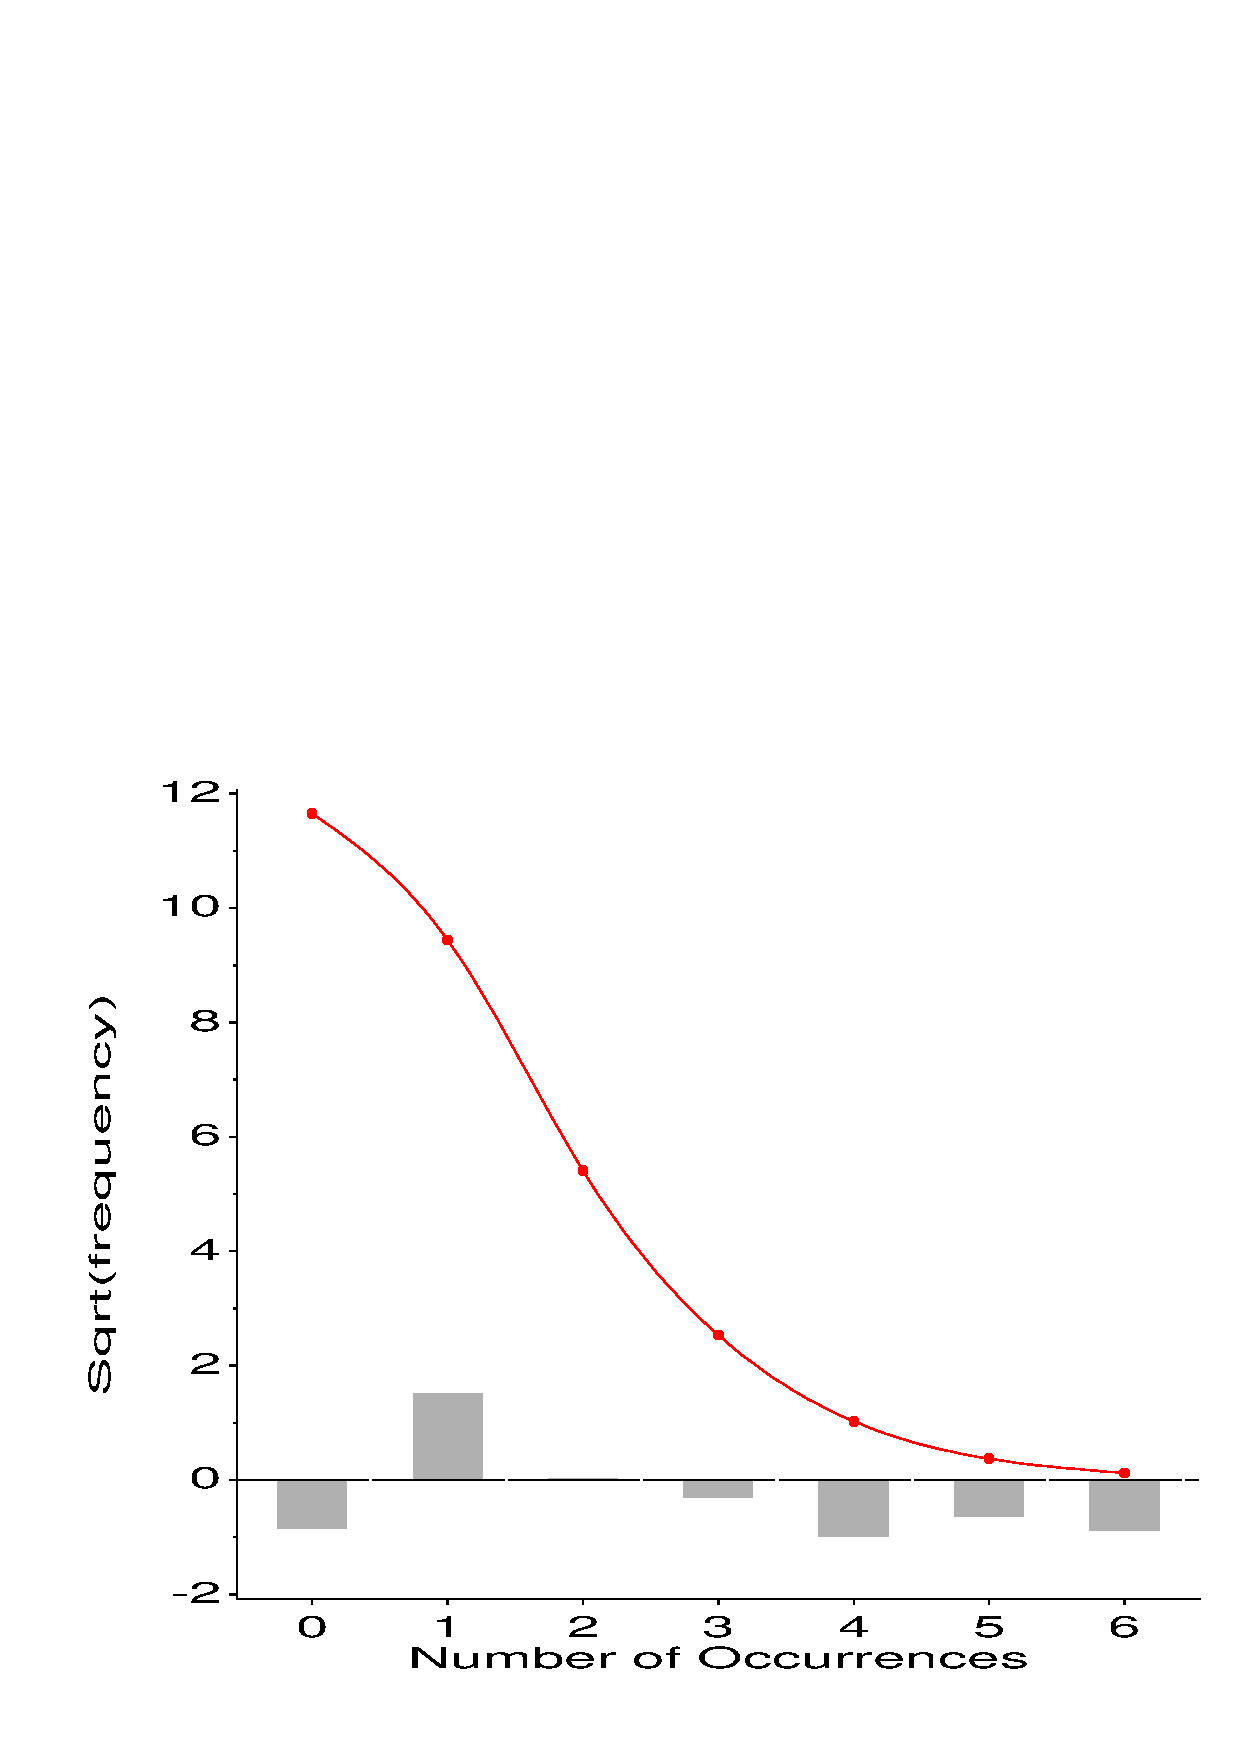
\includegraphics{madfit4}\graphicsfile{ch2/fig/madfit4.eps}{}
 }
 \end{subfigmatrix}
 \caption[Plots of observed and fitted frequencies]{Plots of observed and fitted frequencies
 for the Federalist Papers data, Poisson model.  Each panel shows the fitted frequencies as a smooth
 curve and observed frequencies as a bar.  Panel (a) raw frequencies;
 panels (b)-(d) on a square-root scale, to emphasize smaller frequencies.  Panel (c) is a hanging rootogram, where observed - fitted differences can be judged relative to the horizontal line. Panel (d) shows only the difference between the observed and fi

tted frequency.}\label{fig:madfit}
\end{figure}

